%!TEX TS-program = xelatex
\documentclass[eforms]{EdipyLabs} % Custom class provided for EDIPY labs.
\SetLabNumber{9}
\SetLabTitle{Πρωτόκολλα Επικαλύπτοντος Δέντρου (STP)}
\SetAuthor{Χρήστος Δαλαμάγκας}
\SetLabDescription{Επικαλυπτόμενο Δέντρο (Spanning Tree), STP, RSTP, 802.1D, 802.1w, PVST+, Rapid PVST+.}
\SetLabPrerequisites{Εργαστηριακό φυλλάδιο 08 (VLAN).}

\begin{document}
\Initialize

\section*{Εισαγωγή}
Αντικείμενο του παρόντος εργαστηριακού φυλλαδίου αποτελεί η μελέτη του πρωτοκόλλου STP και των παραλλαγών του. Η γενική άποψη της τοπολογίας που θα υλοποιήσετε στο πλαίσιο της εργαστηριακής άσκησης φαίνεται στο σχήμα \ref{fig:generic}. Η εργαστηριακή άσκηση αποτελείται από δυο σενάρια, με το πρώτο να καλύπτει την παραμετροποίηση του PVST+ και το δεύτερο να επικεντρώνεται στο Rapid PVST+ και την υλοποίηση των βέλτιστων πρακτικών για τη ρύθμιση δικτύων μεταγωγής με το STP. 

\begin{figure}[ht]
	\centering
	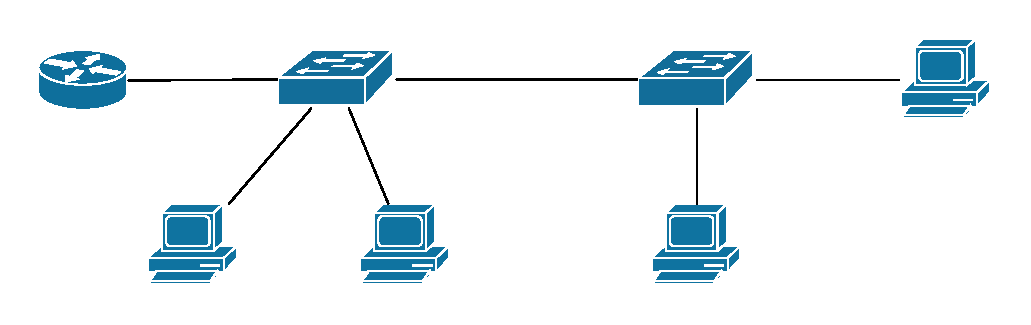
\includegraphics[width=0.75\linewidth]{generic-topology}
	\caption{Η γενική άποψη της τοπολογίας προς υλοποίηση.}\label{fig:generic}
\end{figure}

Για την υλοποίηση της τοπολογίας θα χρειαστείτε τις εξής συσκευές:
\begin{itemize}
	\item x2 Cisco Catalyst 2960.
	\item x1 Cisco 2921.
	\item x4 υπολογιστές.
\end{itemize}

\section{Θεωρητικό υπόβαθρο}

Ο πλεονασμός διαδρομών (redundancy) είναι ένας από τους πιο κοινούς τρόπους για την αύξηση της αξιοπιστίας και της διαθεσιμότητας ενός δικτύου, παράγοντας ιδιαίτερα σημαντικός σε παραγωγικά περιβάλλοντα. Η μέθοδος αυτή επιτρέπει την παροχή εναλλακτικών διαδρομών σε περίπτωση που κάποια συσκευή ή μεμονωμένη διαδρομή αποτύχει. Για τη σχεδίαση μιας τέτοιας τοπολογίας προστίθενται επιπλέον ζεύξεις μεταξύ των συσκευών, ακόμη και νέες συσκευές, οι οποίες προσφέρουν εναλλακτικά μονοπάτια, τα οποία ενεργοποιούνται όταν οι κύριες διαδρομές αποτύχουν. 

Παράδειγμα εφεδρικότητας παρατίθεται στο σχήμα \ref{fig:generic}, στο οποίο o PC1 μπορεί να επικοινωνήσει με τον PC3 είτε μέσω του S1 και του S3 ή μέσω των S1, S2 και S3. Στην περίπτωση που η σύνδεση των S1 και S3 αποτύχει, λόγω της καταστροφής του φυσικού καλωδίου ή μιας εκ των θυρών για παράδειγμα, τα πλαίσια μπορούν να προωθηθούν μέσω του S2.

H τοπολογία του σχήματος \ref{fig:generic} μπορεί να προκαλέσει αρκετά προβλήματα, λαμβάνοντας υπόψιν τον τρόπο που λειτουργούν οι μεταγωγείς και το γεγονός ότι τα πλαίσια ethernet δεν διαθέτουν πεδίο Time-To-Live (TTL), άρα μπορούν να κινούνται αενάως σε ένα δίκτυο. Για παράδειγμα, έστω ότι ο PC1 στέλνει ένα πλαίσιο ευρυεκπομπής. Αρχικά, το πλαίσιο φτάνει στον S1, ο οποίος ενημερώνει τον πίνακα MAC του με τη θύρα εισόδου του πλαισίου και τη MAC του PC1 και προωθεί το πλαίσιο προς τον S2 και τον S3. Οι δυο μεταγωγείς ενημερώνουν τον πίνακα MAC τους και προωθούν το πλαίσιο προς όλες τους τις θύρες, εκτός από αυτήν που το έλαβαν. Δηλαδή, ο S3 προωθεί το πλαίσιο προς τον PC3 και τον S2, ενώ ο S2 προωθεί το πλαίσιο στον S3. Συνεπώς, οι δυο μεταγωγείς λαμβάνουν ξανά το ίδιο πλαίσιο ευρυεκπομπής από άλλη θύρα και το προωθούν από όλες τις άλλες θύρες τους, εκτός από αυτήν από την οποία το έλαβαν. Αυτή η διαδικασία έχει ως συνέπεια τα πλαίσια να «παγιδεύονται» στον βρόχο μεταξύ των μεταγωγέων και νομοτελειακά οι πόροι να εξαντληθούν και το δίκτυο να καταρρεύσει.

Τα προβλήματα που παρατηρούνται στην παραπάνω διαδικασία συνοψίζονται στα εξής:
\begin{itemize}
	\item \textbf{Αστάθεια πίνακα MAC} (MAC database instability): Οι μεταγωγείς ενημερώνουν συνεχώς τον πίνακα MAC, αφού λαμβάνουν το ίδιο πλαίσιο από διαφορετικές θύρες.
	\item \textbf{Καταιγίδες ευρυεκπομπών} (Broadcast storms): Οι μεταγωγείς επαναπροωθούν τα πλαίσια ευρυεκπομπής που λαμβάνουν, με συνέπεια αυτά να καταναλώνουν όλους τους διαθέσιμους πόρους και να είναι αδύνατη η προώθηση της επιθυμητής κίνησης. Η εν λόγω καταιγίδα είναι μια αποτελεσματική μέθοδος άρνησης εξυπηρέτησης (Denial of Service - DoS).
	\item \textbf{Διπλότυπα πλαίσια μονοεκπομπής} (Duplicate unicast frames): Οι υπολογιστές λαμβάνουν πολλαπλά αντίγραφα των πλαισίων που προορίζονται για τους ίδιους. Πρωτόκολλα και υπηρεσίες ανώτερων επιπέδων δεν είναι σχεδιασμένα για να αναγνωρίζουν πανομοιότυπα δεδομένα που έρχονται πολλαπλές φορές.~
\end{itemize} 
Την εγγενή αδυναμία του πρωτοκόλλου ethernet να περιορίζει την αέναη μετάδοση πλαισίων αντιμετωπίζει το πρωτόκολλο επικαλύπτοντος δέντρου (Spanning Tree Protocol - STP). Το πρωτόκολλο απαλείφει τους βρόγχους εφαρμόζοντας τον αλγόριθμο επικαλύπτοντος δέντρου (Spanning Tree Algorithm - SPA) για τον υπολογισμό του ελάχιστου επικαλυπτόμενου δέντρου (Minimum Spanning Tree - MST) μιας τοπολογίας, μπλοκάροντας επιλεκτικά πλεονάζουσες θύρες των μεταγωγέων που δημιουργούν τους βρόχους. 

\subsection{Λειτουργία του STP}

Για την εξάλειψη των βρόχων σε ένα δίκτυο ethernet, οι μεταγωγείς που βρίσκονται στον ίδιο τομέα ευρυεκπομπής ανταλλάσσουν μηνύματα με σκοπό να εκλέξουν έναν μεταγωγέα ως κοινό σημείο αναφοράς και στην συνέχεια να επιλέξουν τη θύρα που οδηγεί στο κοινό σημείο αναφοράς με το μικρότερο κόστος, μπλοκάροντας ταυτόχρονα άλλες θύρες που προκαλούν βρόχο.

\notebox{Υπάρχουν πολλές παραλλαγές του πρωτότυπου STP που χρησιμοποιούνται σήμερα. Στο παρόν φυλλάδιο, η αναφορά στο STP αφορά την προτυποποίηση 802.1D-1998, η οποία είναι προεπιλογή για τις συσκευές Cisco.}

\begin{figure}[ht]
	\centering
	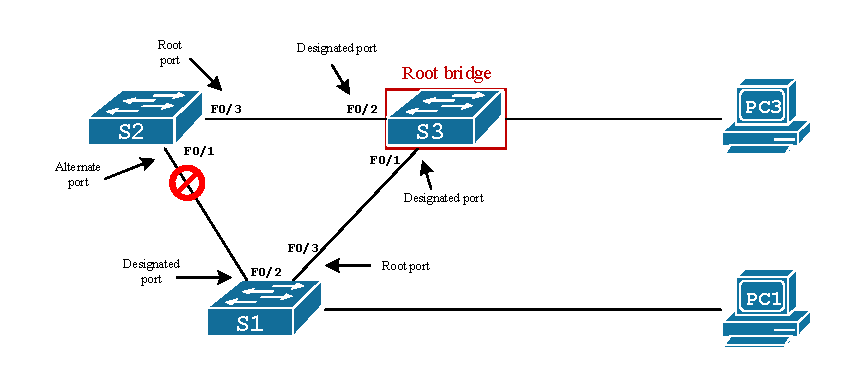
\includegraphics[width=\linewidth]{stp-function}
	\caption{Παράδειγμα ομαδοποίησης υπολογιστών σε VLAN.}\label{fig:stp}
\end{figure}

Για το STP χρησιμοποιείται η εξής ορολογία, η οποία απεικονίζεται στο σχήμα \ref{fig:stp}:
\begin{itemize}
	\item \textbf{Root bridge}: Είναι εκείνος ο μεταγωγέας που χρησιμοποιούν όλοι οι άλλοι μεταγωγείς του ίδιου τομέα ευρυεκπομπής ως αναφορά για τον υπολογισμό του MST. Ως root bridge εκλέγεται ο μεταγωγέας με το μικρότερο bridge ID και καμία θύρα του δε μπλοκάρεται από το STP.
	\item \textbf{Root port}: Είναι η θύρα κάθε μεταγωγέα που οδηγεί στο root bridge με το μικρότερο κόστος. Ένας μεταγωγέας root bridge δεν έχει root port. 
	\item \textbf{Designated port}: Θύρα η οποία μπορεί να οδηγήσει στο root bridge και δεν έχει μπλοκαριστεί από το STP.
	\item \textbf{Alternate port}: Εναλλακτική θύρα, η οποία μπορεί να οδηγήσει στο root bridge και έχει μπλοκαριστεί από το STP για την αποφυγή βρόχου.  
	\item \textbf{Bridge ID} (BID): Είναι ένας αριθμός 8 byte που καθορίζει την εκλογή του root bridge και του ρόλου των θυρών του μεταγωγέα. Στο σχήμα \ref{fig:bid} απεικονίζεται η μορφή αυτού του αριθμού και περιγράφεται ως εξής:
	\begin{itemize}
		\item \textbf{Priority}: Τα πρώτα 4 bit διαμορφώνουν την προτεραιότητα ενός μεταγωγέα στην εκλογή. Αυτός με τη \textbf{χαμηλότερη} προτεραιότητα αναδεικνύεται ως root bridge. Προεπιλεγμένη τιμή του αριθμού αυτού είναι ${1000}_{(2)}$ ή $32768$. Η τιμή του μπορεί να αλλάξει χειροκίνητα, θα πρέπει ωστόσο να είναι πολλαπλάσια του 4096.
		\item \textbf{Extended System ID}: Επειδή ο μεταγωγέας ενδέχεται να συμμετέχει σε πολλές διαδικασίες εκλογής, αν οι θύρες του ανήκουν σε πολλά VLAN, ο αριθμός αυτός μεγέθους 12 bit εξασφαλίζει ότι ο μεταγωγέας θα έχει διαφορετική προτεραιότητα σε κάθε VLAN. Απο προεπιλογή, η τιμή του είναι~1.
		\item \textbf{MAC address}: Τα τελευταία 48 bit του αριθμού συμπληρώνει η διεύθυνση MAC του μεταγωγέα (base ethernet MAC), την οποία μπορεί να δει κάποιος με την εντολή \ip{show version}.
	\end{itemize}
	\item \textbf{Κόστος θύρας} είναι αυτό που θεωρεί ο STA ως κόστος για τη διάσχιση μιας θύρας. Το κόστος εξαρτάται από την ταχύτητα της θύρας και λαμβάνεται υπόψιν για την επιλογή της root port. Τα προεπιλεγμένα κόστη παρατίθενται στον πίνακα \ref{tab:costs}
	\item \textbf{Bridge Protocol Data Unit} (BPDU): Είναι τα μηνύματα που ανταλλάσσουν οι μεταγωγείς για τον καθορισμό του root bridge και τον ρόλων των θυρών. Μεταξύ των 12 πεδίων του μηνύματος, περιέχεται \begin{enumerate*} \item[\textbf{α)}] το τρέχων BID του root bridge (\textbf{root ID}) \item[\textbf{β)}] το συνολικό κόστος του μεταγωγέα για να φτάσει στο root bridge (\textbf{root path cost}) \item[\textbf{γ)}] την τιμή του χρονόμετρου hello time\end{enumerate*}.
	\item \textbf{Χρονόμετρα}: Το STP χρησιμοποιεί τα εξής χρονόμετρα: 
	\begin{itemize}
		\item \textbf{Hello time} (2 δευτερόλεπτα) είναι το μεσοδιάστημα αποστολής BPDU από το root bridge. 
		\item \textbf{Forwarding time} (15 δευτερόλεπτα) είναι το χρονικό διάστημα παραμονής στις καταστάσεις listening και learning.
		\item \textbf{Max age} (20 δευτερόλεπτα) είναι η μέγιστη διάρκεια ζωής μιας πληροφορίας BPDU για έναν απομακρυσμένο μεταγωγέα. Το χρονόμετρο αυτό ανανεώνεται κάθε φορά που λαμβάνεται ένα BPDU από έναν απομακρυσμένο μεταγωγέα. Αν το χρονόμετρο λήξει χωρίς να ληφθεί BPDU από έναν απομακρυσμένο μεταγωγέα, τότε διαγράφονται όλες οι πληροφορίες BPDU για τον απομακρυσμένο μεταγωγέα, θεωρώντας οτι είναι εκτός δικτύου, και εκτελείται ξανά το STP, αν είναι απαραίτητο.
	\end{itemize}
	\begin{figure}[ht]
		\centering
		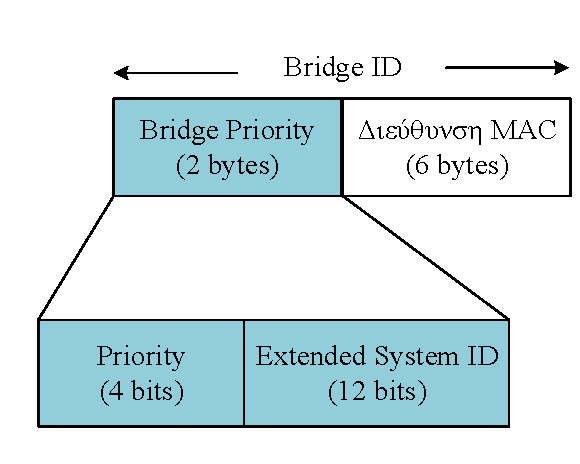
\includegraphics[width=0.45\linewidth]{bid}
		\caption{Παράδειγμα ομαδοποίησης υπολογιστών σε VLAN.}\label{fig:bid}
	\end{figure}
\end{itemize}

Το STP εκτελείται αμέσως μετά την εκκίνηση του λειτουργικού συστήματος. Αν όλες οι θύρες του κάθε μεταγωγέα ξεκινήσουν να προωθούν πλαίσια, πριν υπολογιστεί πλήρως το MST, ενδέχεται να προκληθεί προσωρινά βρόχος. Γιαυτό, το STP χρησιμοποιεί πέντε διαφορετικές καταστάσεις θυρών που διασφαλίζουν πως δεν δημιουργείται βρόχος κατά τη δημιουργία του MST. Οι καταστάσεις παρατίθενται συνοπτικά στον πίνακα \ref{tab:port-states}:

\begin{itemize}
	\item \textbf{Blocking}: Στην κατάσταση αυτή εισέρχεται κάθε ενεργή θύρα με την εκκίνηση της διαδικασίας εκλογής. Η θύρα δεν δέχεται κανένα άλλο πλαίσιο, παρά μόνο μηνύματα BPDU, τα οποία και επεξεργάζεται ο μεταγωγέας για τη λήψη αποφάσεων σχετικά με τον ρόλο των θυρών του.
	\item \textbf{Listening}: Μετά από 20 δευτερόλεπτα, οι θύρες designated και root μεταβαίνουν σε αυτήν την κατάσταση. Η συμπεριφορά των θυρών είναι ίδια με αυτήν της κατάστασης blocking.  
	\item \textbf{Learning}: Έπειτα από 15 δευτερόλεπτα, οι θύρες listening μεταβαίνουν στην κατάσταση learning, κατά την οποία ο μεταγωγέας επεξεργάζεται τα πλαίσια δεδομένων που δέχεται, ενημερώνοντας τον πίνακα MAC. Παρόλα αυτά, ο μεταγωγέας δεν προωθεί τα πλαίσια που λαμβάνει από τις θύρες learning. 
	\item \textbf{Forward}: Έπειτα από 15 δευτερόλεπτα, οι θύρες learning εισέρχονται στην κατάσταση forwarding. Η κατάσταση αυτή είναι η κανονική, κατά την οποία η θύρα συμμετέχει πλήρως στην τοπολογία.
	\item \textbf{Disabled}: Η θύρα σε αυτή την κατάσταση δεν συμμετέχει στην διαδικασία του STP, διότι είναι εκτός λειτουργίας.
\end{itemize}



\begin{table}[ht]\renewcommand\arraystretch{1.5}
	\rowcolors{2}{white}{lightgray}\centering
		\begin{tabular}{lccccc}\FormatFirstRow
			 				& \multicolumn{5}{c}{\textbf{Κατάσταση θύρας}}                      \\
			\rowcolor{gray!50}
			\multirow{-2}{*}{\textbf{Επιτρεπόμενη ενέργεια}}	& \textbf{Blocking} & \textbf{Listening} & \textbf{Learning} & \textbf{Forward} & \textbf{Disabled} \\
			Επεξεργασία BPDU   & \textcolor{ForestGreen}{\faCheck}  & \textcolor{ForestGreen}{\faCheck}         	 & \textcolor{ForestGreen}{\faCheck}          & \textcolor{ForestGreen}{\faCheck}        	& \textcolor{BrickRed}{\faTimes}          \\
			Προώθηση εισερχομένων δεδομένων    & \textcolor{BrickRed}{\faTimes}         	& \textcolor{BrickRed}{\faTimes}            & \textcolor{BrickRed}{\faTimes}           & \textcolor{ForestGreen}{\faCheck}         & \textcolor{BrickRed}{\faTimes}         \\
			Εκμάθηση διευθύνσεων MAC           & \textcolor{BrickRed}{\faTimes}         	& \textcolor{BrickRed}{\faTimes}           & \textcolor{ForestGreen}{\faCheck}          & \textcolor{ForestGreen}{\faCheck}        	& \textcolor{BrickRed}{\faTimes}         
		\end{tabular}
	\caption{Οι καταστάσεις θυρών στο STP.}\label{tab:port-states}
\end{table}

Συνοπτικά, λοιπόν, το STP παρέχει ένα MST χωρίς βρόχους εκτελώντας τα εξής βήματα:
\begin{itemize}
	\item \textbf{Εκλογή} root bridge: Με την εκκίνηση του λειτουργικού του συστήματος, κάθε μεταγωγέας στέλνει μήνυματα BPDU προς τους γειτονικούς μεταγωγείς του θεωρώντας πως ο ίδιος είναι root bridge. Στα μηνύματα αυτά ο μεταγωγέας ενσωματώνει το δικό του BID, καθώς και το root ID που έχει ορίσει, το οποίο αρχικά ταυτίζεται με το BID. Οι γειτονικοί μεταγωγείς συγκρίνουν το δικό τους root ID με τα BID που λαμβάνουν και αν λάβουν κάποιο BID με μικρότερη τιμή, τότε αλλάζουν το root ID τους με το μικρότερο.
	\item \textbf{Επιλογή θύρας root}: Για να αποφασίσει ένας μεταγωγέας ποια από τις θύρες του θα ορίσει ως root port, κάνει τις εξής συγκρίσεις:
	\begin{enumerate}
	\item Στο πεδίο root path cost κάθε εισερχόμενου BPDU προστίθεται το κόστος της θύρας από την οποία εισήλθε αυτό (ingress port). Θύρα root γίνεται αυτή από την οποία προέκυψε το μικρότερο αθροιστικό κόστος. 
	\item Αν τα κόστη βγαίνουν ίδια για κάθε θύρα που συμμετέχει στο STP, τότε ο μεταγωγέας επιλέγει τη θύρα από την οποία έλαβε BPDU με το χαμηλότερο bridge ID.
	\item Τέλος, αν τα bridge ID των BPDU που λαμβάνονται από όλες τις θύρες είναι τα ίδια (αυτό συμβαίνει όταν συνδέονται δυο μεταγωγείς με δυο ή περισσότερα καλώδια), τότε root γίνεται η θύρα που \textbf{έλαβε} BPDU από θύρα με το χαμηλότερο port priority. 
	\end{enumerate}
	\item \textbf{Ορισμός θυρών designated και alternate}: Μια θύρα root έχει πάντα απέναντί της μια θύρα designated. Όταν βρίσκονται απέναντι δυο θύρες non-root, τότε αυτή που ανήκει στον μεταγωγέα με το χαμηλότερο bridge ID τίθεται σε κατάσταση forwarding (designated) και η απέναντι σε κατάσταση blocking (alternate). Αν τα bridge ID είναι τα ίδια, τότε λαμβάνεται υπόψιν το χαμηλότερο port-priority που λαμβάνεται.
\end{itemize}

\begin{table}[ht]\renewcommand\arraystretch{1.5}
	\centering
	\rowcolors{2}{lightgray}{white}
		\begin{tabular}{lll}\FormatFirstRow
			\textbf{Ρυθμός μετάδοσης} & \textbf{Κόστος για STP/PVST+} 	 & \textbf{Κόστος για RSTP/Rapid PVST+}\\
			10 Mbit/s				  & 100		 	 			 & $2\ 000\ 000$ \\ 
			100 Mbit/s				  & 19		   				 & $200\ 000$ \\
			1 Gbit/s			 	  & 4			   			 & $20\ 000$ \\
			10 Gbit/s 				  & 2 		   				 & $2\ 000$
		\end{tabular}
	\caption{Τα κόστη διάσχισης των θυρών για το STP και το RSTP.}\label{tab:costs}
\end{table}

\notebox{Παρόλο που το STP λειτουργεί χωρίς την επέμβαση του διαχειριστή, είναι συνήθης πρακτική σε παραγωγικά περιβάλλοντα η χειροκίνητη αλλαγή του bridge priority των μεταγωγέων για τον επηρεασμό της διαδικασίας εκλογής root bridge. Συνήθως, τα παλαιότερα μοντέλα μεταγωγέων έχουν μικρότερη διεύθυνση MAC, άρα προκρίνονται στην εκλογή root bridge, κάτι το οποίο μπορεί να μην είναι η βέλτιστη επιλογή. Η χειροκίνητη αλλαγή της προτεραιότητας μπορεί να προκρίνει ένα καλύτερο μοντέλο μεταγωγέα ως root bridge.}

\subsection{Παραλλαγές του STP}

\begin{table}[ht]\renewcommand\arraystretch{1.5}
	\centering\rowcolors{2}{lightgray}{white}
	\begin{tabular}{lllll}\FormatFirstRow
		\textbf{Πρωτόκολλο} & \textbf{Πρότυπο} & \textbf{Απαίτηση σε πόρους} & \textbf{Σύγκλιση} & \textbf{Υποστήριξη VLAN}\\
		STP			& 802.1D-1998		   & Χαμηλή						 & Αργή				 & Όχι\\
		RSTP				& 802.1D-2004		   & Μεσαία						 & Γρήγορη			 & Ναι\\
		PVST+				& Cisco (802.1D-1998)			   & Υψηλή						 & Αργή				 & Όχι\\
		Rapid PVST+ 		& Cisco (802.1D-2004) 		   & Πολύ υψηλή					 & Γρήγορη			 & Ναι\\
		MSTP/MST		 & 802.1s, Cisco	   & Υψηλή						 & Γρήγορη			 & Ναι, βελτιωμένη
	\end{tabular}
	\caption{Συγκριτική παράθεση των παραλλαγών του STP.}\label{tab:comparison}
\end{table}


To πρώτο έγγραφο για την προτυποποίηση του STP δημοσιεύτηκε από την IEEE το 1990 υπό την ονομασία 802.1D. Έκτοτε έχουν εκδοθεί οι εξής εκδόσεις, οι οποίες συνοψίζονται στον πίνακα \ref{tab:comparison}: 
\begin{itemize}
	\item \textbf{Spanning Tree Protocol} (STP 802.1D-1998): Πρόκεται για τροποποίηση της πρωτότυπης έκδοσης του STP από την ΙΕΕΕ. Αν και η έκδοση του προτύπου έχει αντικατασταθεί από την IEEE, το 802.1D-1998 χρησιμοποιείται ακόμα από πολλές δικτυακές συσκευές. 
	\item \textbf{Per-VLAN Spanning Tree Plus} (PVST+): Είναι η υλοποίηση του STP 802.1D-1998 από τη Cisco και \textbf{προεπιλογή} για τις συσκευές της. Χαρακτηριστικά της υλοποίησης είναι η διατήρηση ξεχωριστής διεργασίας και δέντρου STP για κάθε VLAN της τοπολογίας και διάφορες βελτιώσεις, όπως PortFast και BPDU guard.
	\item \textbf{Rapid Spanning Tree Protocol} (RSTP): Το πρωτόκολλο συμπεριλαμβάνεται στο 802.1D-2004 και επίσημα έχει αντικαταστήσει το STP. To RSTP μείωσε τους ρόλους των θυρών σε τρείς και εισήγαγε την έννοια της θύρας edge, αντίστοιχη με το PortFast του PVST+.
	\item \textbf{Rapid PVST+}: Είναι η υλοποίηση του RSTP από τη Cisco. Στη λογική του PVST+, υποστηρίζει διαφορετική διεργασία RSTP και δέντρο ανά VLAN, καθώς και τις βελτιώσεις του PVST+ (PortFast, BPDU guard κλπ).
	\item \textbf{Multiple Spanning Tree Protocol} (MSTP/MST): To πρότυπο της IEEE (MSTP) και η αντίστοιχη υλοποίηση της Cisco (MST) υποστηρίζουν τη δυναμική ομαδοποίηση VLAN σε διεργασίες και δέντρα RSTP, ανάλογα με τα χαρακτηριστικά της κίνησής τους.

\end{itemize}

Σήμερα, τα ανοιχτά πρότυπα της IEEE έχουν συμπεριληφθεί στο πρότυπο 802.1Q-2018, το οποίο συμπεριλαμβάνει όλα τα πρωτόκολλα και τις υπηρεσίες που χρησιμοποιούνται στο ethernet.   

\subsection{PortFast και BPDU guard}
To PortFast είναι ένα χαρακτηριστικό των υλοποιήσεων τύπου PVST+, βελτίωση του πρωτότυπου STP 802.1D-1998 από την IEEE, που επιτρέπει την απευθείας μετάβαση των θυρών σε κατάσταση forwarding, παραβλέποντας τις καταστάσεις listening και learning. Το PortFast μπορεί να ενεργοποιηθεί σε οποιαδήποτε θύρα σε κατάσταση πρόσβασης (access port), δηλαδή σε θύρα στην οποία συνδέεται ένας εξυπηρετητής ή ένα τερματικό.

Μια θύρα που έχει οριστεί ως PortFast, δεν επιτρέπεται να λάβει πλαίσιο BPDU. Αν μια θύρα PortFast λάβει BPDU, σημαίνει ότι συνδέθηκε σε αυτήν ένας μεταγωγέας, ο οποίος μπορεί να προκαλέσει βρόχο. Η Cisco υποστηρίζει τη λειτουργία BPDU guard για τις θύρες PortFast, η οποία ενεργοποιείται όταν μια θύρα PortFast λάβει πλαίσιο BPDU. Αποτέλεσμα της λειτουργίας BPDU guard είναι να απενεργοποιήσει διαχειριστικά τη διεπαφή ώστε να αποτραπεί ενδεχόμενη δημιουργία βρόχου. Από προεπιλογή, οι λειτουργίες PortFast και BPDU guard είναι απενεργοποιημένες.

\notebox{Η τεχνολογία PortFast επιτρέπει την ομαλή λειτουργία υπηρεσιών, όπως το DHCP και το Preboot eXecution Environment (PXE) για εκκίνηση λειτουργικού συστήματος μέσω δικτύου. Χωρίς το PortFast, οι υπολογιστές ρυθμισμένοι ως πελάτες DHCP, δεν λαμβάνουν εγκαίρως διεύθυνση IP, με αποτέλεσμα, στην περίπτωση του PXE, να συμβεί time-out και το UEFI να εκκινήσει το λειτουργικό σύστημα του σκληρού δίσκου αντί του λειτουργικού συστήματος από τον εξυπηρετητή PXE. Συνίσταται, λοιπόν, ειδικά σε περιβάλλοντα PXE, να ενεργοποιείται η λειτουργία PortFast.}
\newpage

\subsection{Επισκόπηση του RSTP} 

Οι κυριότερες αλλαγές που εισήγαγε το RSTP, τις οποίες έχει υιοθετήσει και το Rapid PVST+, συνοψίζονται στις εξής:
\begin{itemize}
	\item Οι καταστάσεις, Disabled, Blocking και Listening του STP συγχωνεύτηκαν στην κατάσταση \textbf{Discarding} του RSTP. Έτσι, το RSTP καθίσταται πλήρως συμβατό με το STP.
	\item Στο STP, μόνο ο root bridge στέλνει μηνύματα BPDU κάθε hello time. Αντίθετα, στο RSTP κάθε μεταγωγέας στέλνει μηνύματα BPDU κάθε hello time, επιτρέποντας τη γρηγορότερη διάδοση κάποιας αλλαγής στην τοπολογία.
	\item \textbf{Edge ports}: Οι θύρες αυτού του είδους δεν συνδέονται με κάποιον μεταγωγεα, συνεπώς, επιτρέπεται η απευθείας μετάβασή τους σε κατάσταση forwarding.
	\item \textbf{Link types}: To RSTP υποστηρίζει δυο είδη θυρών ανάλογα με την αμφιδρομικότητα της θύρας, point-to-point αν η θύρα είναι πλήρως αμφίδρομη και shared αν είναι ημιαμφίδρομη.
\end{itemize}
Στον πίνακα που ακολουθεί συνοψίζονται οι καταστάσεις των θυρών στο STP και το RSTP:

\begin{table}[ht]\renewcommand\arraystretch{1.5}%\rowcolors{2}{lightgray}{white}
	\resizebox{\textwidth}{!}{
	\begin{tabular}{llll}\FormatFirstRow
	\textbf{Κατάσταση θύρας STP} 	& \textbf{Κατάσταση θύρας RSTP} & \textbf{Εντάσσεται στην τοπολογία;} & \textbf{Μαθαίνει διευθύνσεις MAC;}\\         	
	Disabled		& 							 	& \textcolor{BrickRed}{\faTimes}		& \textcolor{BrickRed}{\faTimes} \\
	Blocking		& 								& \textcolor{BrickRed}{\faTimes}		& \textcolor{BrickRed}{\faTimes} \\
	Listening		&  \multirow{-3}{*}{Discarding}	& \textcolor{ForestGreen}{\faCheck}		& \textcolor{BrickRed}{\faTimes} \\
\rowcolor{lightgray}
	Learning 		& Learning  					& \textcolor{ForestGreen}{\faCheck}		& \textcolor{ForestGreen}{\faCheck} \\
	Forwarding		& Forwarding					& \textcolor{ForestGreen}{\faCheck}		& \textcolor{ForestGreen}{\faCheck}
\end{tabular}
}
\caption{Καταστάσεις θυρών για STP και RSTP.}\label{tab:comparison2}
\end{table}


\subsection{(Rapid) PVST+ και εξισορρόπηση φόρτου}
O root bridge διαδραματίζει κρίσιμο ρόλο σε ένα δίκτυο μεταγωγής, είναι ο μεταγωγέας/κόμβος στον οποίον συγκεντρώνεται η κίνηση των υπολοίπων μεταγωγέων, με σκοπό να αποτραπεί η δημιουργία βρόχων. Ο ρόλος αυτός ενδέχεται να προκαλέσει σοβαρή επιβάρυνση ή εξάντληση πόρων σε έναν root bridge.

Μια λύση στο πρόβλημα της επιβάρυνσης του root bridge είναι η εξισορρόπηση του φόρτου αυτού, ορίζοντας διαφορετικό root bridge για κάθε VLAN της τοπολογίας. Για τα πρωτόκολλα που διατηρούν διαφορετική διεργασία και δέντρο για κάθε VLAN, ένας διαχειριστής μπορεί να τροποποιήσει την προτεραιότητα των bridge ID, ώστε να προκύπτει διαφορετικός μεταγωγέας ως root bridge για κάθε VLAN.

\newpage
\section{Προετοιμασία δικτύου}\label{sec:2}

\begin{figure}[H]
	\centering
	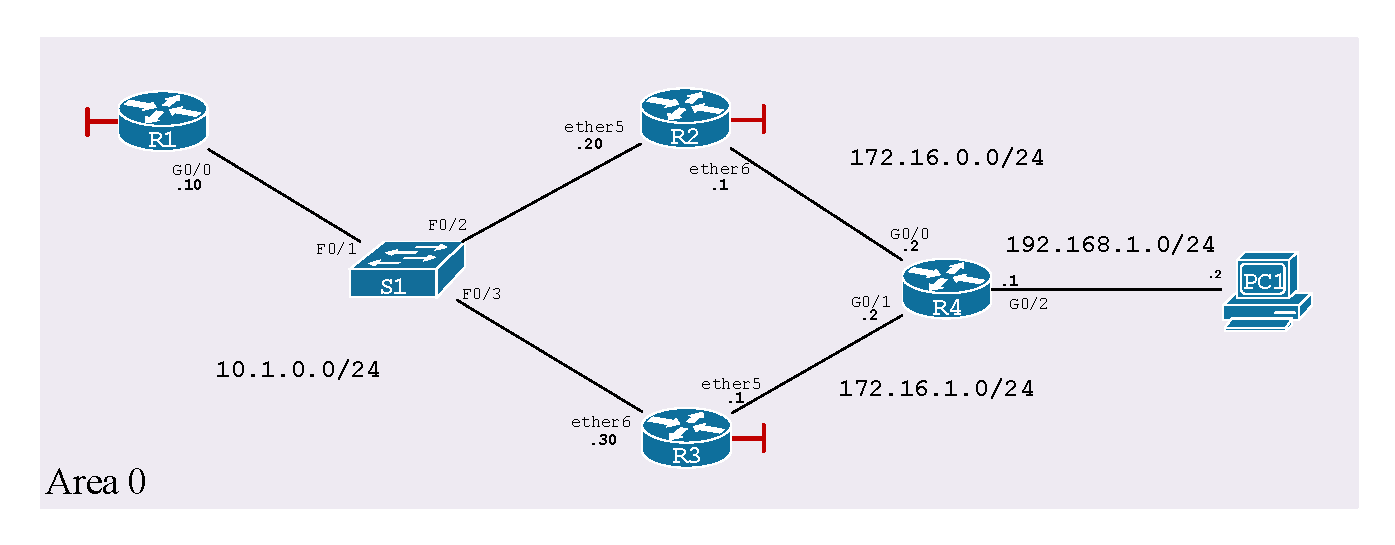
\includegraphics[width=\linewidth]{topology-1}
	\caption{Το σχέδιο της αναλυτικής τοπολογίας προς υλοποίηση.}\label{fig:topology-1}
\end{figure}

\begin{table}[H]
	\centering\renewcommand{\arraystretch}{1.1}
		\begin{tabular}{c>{\bfseries\ttfamily}c>{\bfseries\ttfamily}l>{\bfseries\ttfamily}l}
			\FormatFirstRow
			\normalfont\textbf{Συσκευή} & \normalfont\textbf{Διεπαφή} & \normalfont\textbf{Διεύθυνση IP} & \normalfont\textbf{Μάσκα υποδικτύου} \\
			S1							& \SVI						  & 192.168.88.1				 	 &  255.255.255.0   \\
			\rowcolor{lightgray}
			S2							& \SVI						  & 192.168.88.2					 &  255.255.255.0   \\
			S3							& \SVI						  & 192.168.88.3					 &  255.255.255.0   \\
			\rowcolor{lightgray}
			PC1							& \NIC						  & 192.168.10.1					 &  255.255.255.0   \\
			PC3							& \NIC						  & 192.168.10.3					 &  255.255.255.0   
		\end{tabular}
	\caption{Το σχήμα διευθυνσιοδότησης της τοπολογίας.}\label{tab:iptable-1}
\end{table}

\begin{VlanTable}{Το σχήμα ανάθεσης VLAN.}{vlantable-1}
												&							& S1: \ip{Fa0/0/18}\\
	\multirow{-2}{*}{10}						& \multirow{-2}{*}{User} 	& S3: \ip{Fa0/0/6} \\
	\rowcolor{lightgray}    
	88											& Management				& S1, S2, S3: SVI
\end{VlanTable}
\newpage
Ακολουθήστε τα εξής βήματα για την προετοιμασία του δικτύου της εργαστηριακής άσκησης:
\begin{itemize}
	\item Υλοποιήστε τη συνδεσμολογία που απεικονίζεται στο σχήμα της τοπολογίας.
	
	\importantbox{Για αρχή, συνδέστε τους μεταγωγείς μεταξύ τους με \textbf{ένα} καλώδιο. Για τη σύνδεση S1 με S2 χρησιμοποιήστε τις θύρες F0/0/2 και F0/0/2, για τους S1 με S3 τις θύρες F0/0/4 και F0/0/4 και για τους S2 και S3 τις θύρες F0/0/4 και F0/0/2.}
	
	\item Βεβαιωθείτε ότι οι δικτυακές συσκευές λειτουργούν στις εργοστασιακές ρυθμίσεις.
	\item Αναθέστε διευθύνσεις IP στους υπολογιστές και τις SVI των μεταγωγέων, σύμφωνα με το σχήμα διευθυνσιοδότησης.
	\item Υλοποιήστε το σχήμα ανάθεση VLAN που παρατίθεται στον πίνακα \ref{tab:vlantable-1}. Παράλληλα, ορίστε ως συγκανάλωση τις θύρες που διασυνδέουν τους μεταγωγείς.
\end{itemize}

\section{Σενάριο: PVST+ με πλεονάζοντα μονοπάτια}
Στο πρώτο σενάριο θα παρατηρήσετε τη διαδικασία εκλογής στο PVST+ και θα την επηρεάσετε αλλάζοντας κόστος και προτεραιότητα. Τέλος, θα ενεργοποιήσετε επιπλέον πλεονάζοντα μονοπάτια και θα παρατηρήσετε τις αλλαγές στην διαδικασία επιλογής θύρας root.

\subsection{Καταγραφή ρόλων STP}

Ξεκινώντας, καταγράψτε στον πίνακα \ref{tab:states-1} το bridge ID, τον ρόλο της κάθε θύρας (root, alternate, designated), καθώς και το root bridge της τοπολογίας. Αναγράψτε το bridge ID ως XXXXX.YYYYYY, όπου ΧΧΧΧ το bridge priority, που προκύπτει από το άθροισμα του priority με το extended system ID, και ΥΥΥΥΥΥ η διεύθυνση MAC του μεταγωγέα.

\begin{table}[ht]\centering
	\rowcolors{2}{lightgray}{white}
	\renewcommand{\arraystretch}{1.5}
	\begin{tabular}{lccc}\FormatFirstRow
							& \textbf{S1}				 & \textbf{S2}					& \textbf{S3} 				\\
		\textbf{Bridge ID}	& \textField{1}{4cm}{0.5cm}	 & \textField{2}{4cm}{0.5cm}	& \textField{3}{4cm}{0.5cm} \\
		\textbf{Root bridge;}	& \radioButton{a}{10bp}{10bp}{1} & \radioButton{a}{10bp}{10bp}{2} & \radioButton{a}{10bp}{10bp}{3}\\
		\textbf{F0/0/1}		& \textField{4}{4cm}{0.5cm}	 & \textField{5}{4cm}{0.5cm}	& \textField{6}{4cm}{0.5cm}	\\
		\textbf{F0/0/2}		& \textField{7}{4cm}{0.5cm}  & \textField{8}{4cm}{0.5cm} 	& \textField{9}{4cm}{0.5cm}	\\
		\textbf{F0/0/3}		& \textField{10}{4cm}{0.5cm} & \textField{11}{4cm}{0.5cm} 	& \textField{12}{4cm}{0.5cm}\\
		\textbf{F0/0/4}		& \textField{13}{4cm}{0.5cm} & \textField{14}{4cm}{0.5cm} 	& \textField{15}{4cm}{0.5cm}
	\end{tabular}
	\caption{1η καταγραφή πληροφοριών PVST+}\label{tab:states-1}
\end{table}

Τις πληροφορίες του επικαλύπτοντος δέντρου ενός μεταγωγέα μπορείτε να τις ανακτήσετε με την εντολή \ip{show spanning}. Οι μεταγωγείς διατηρούν ξεχωριστή διεργασία για κάθε VLAN που συμμετέχει, οπότε μπορείτε να περιορίσετε τα αποτελέσματα της εντολής μόνο για το VLAN 10 ως εξής:

\begin{CommandBox}
`Switch>\textbf{show spanning vlan 10}\\
	VLAN0010\\
	\tab[0.25cm] Spanning tree enabled protocol ieee\\[-0.25cm]
	\begin{adjustwidth}{0.25cm}{0cm}
		\begin{tabular}{lll}
			\hl{Root ID}& Priority		& 32778											\\
						& Address   	& 0005.5E8B.3568								\\
						& Cost      	& 19 											\\
						& Port      	& 2(FastEthernet0/0/2)							\\
						& Hello Time  	& 2 sec  Max Age 20 sec  Forward Delay 15 sec	\\
		\end{tabular}\\[-0.5cm]
		\begin{tabular}{lll}
			Bridge ID	& Priority		& \hl{32778} (priority 32768 sys-id-ext 10)			\\
						& Address   	& \hl{00D0.BC96.8D63}								\\
						& Hello Time  	& 2 sec  Max Age 20 sec  Forward Delay 15 sec	\\
						& Aging Time    & 20											\\
		\end{tabular}
	\end{adjustwidth}
	
	\begin{tabular}{llllll}
		Interface        & Role 		& Sts 		& Cost      & Prio.Nbr 	& Type\\
		---------------- & ---- 		& --- 		& --------- & --------  & -------------------\\
		\hl{Fa0/0/2}       & \hl{Root}	&\hl{FWD}	& \hl{19}   & \hl{128.2}& P2p\\
		Fa0/0/18           & Desg 		& FWD 		& 19        & 128.18   	& P2p\\
		Fa0/0/4            & Altn 		& BLK 		& 19        & 128.4   	& P2p
	\end{tabular}`
\end{CommandBox}

Στο παραπάνω ενδεικτικό παράδειγμα βλέπετε πως ο μεταγωγέας έχει ως root bridge αυτόν με διεύθυνση MAC 0005.5E8B.3568. Ο ίδιος μεταγωγέας έχει προτεραιότητα 32778, διεύθυνση MAC 00D0.BC96.8D63 και από τις διεπαφές του, η Fa0/2 είναι root port σε κατάσταση forwarding, το κόστος διάσχισης είναι 19 (βλ. πίνακα \ref{tab:costs} σχετικά) και η προτεραιότητα της θύρας είναι 128.2. 

Κατά τη διάρκεια των αλλαγών μπορείτε να ενεργοποιήσετε τη λειτουργία αποσφαλμάτωσης για το STP ώστε να έχετε πλήρη πληροφόρηση σε πραγματικό χρόνο για την επίδραση των εντολών του STP.

\begin{CommandBox}
Switch#`\textbf{debug spanning-tree events}`
...
\end{CommandBox}

\subsection{Επηρεασμός εκλογής root bridge}

Κριτήριο για την εκλογή root bridge αποτελεί η προτεραιότητα του κάθε μεταγωγέα. Επιλέξτε έναν μεταγωγέα non-root και μειώστε του την προτεραιότητα σε 28672 ώστε να τον προκρίνετε στην εκλογή. Χρησιμοποιήστε την εξής εντολή:

\begin{CommandBox}
Switch#`\textbf{configure terminal}`
Switch(config)#`\textbf{spanning-tree vlan 10 priority 28672}`
\end{CommandBox}

Περιμένετε περίπου 30 δευτερόλεπτα για να συγκλίνει ο STA και, έπειτα, καταγράψτε τις αλλαγές στον πίνακα~\ref{tab:states-2}:

\begin{table}[ht]\centering
	\rowcolors{2}{lightgray}{white}
	\renewcommand{\arraystretch}{1.5}
	\begin{tabular}{lccc}\FormatFirstRow
								& \textbf{S1}				 	 & \textbf{S2}					  & \textbf{S3} 				\\
		\textbf{Bridge ID}		& \textField{16}{4cm}{0.5cm}	 & \textField{17}{4cm}{0.5cm} 	  & \textField{18}{4cm}{0.5cm} \\
		\textbf{Root bridge;}	& \radioButton{b}{10bp}{10bp}{1} & \radioButton{b}{10bp}{10bp}{2} & \radioButton{b}{10bp}{10bp}{3}\\
		\textbf{F0/0/1}			& \textField{19}{4cm}{0.5cm}	 & \textField{20}{4cm}{0.5cm}	  & \textField{21}{4cm}{0.5cm}	\\
		\textbf{F0/0/2}			& \textField{22}{4cm}{0.5cm}  	 & \textField{23}{4cm}{0.5cm} 	  & \textField{24}{4cm}{0.5cm}	\\
		\textbf{F0/0/3}			& \textField{25}{4cm}{0.5cm} 	 & \textField{26}{4cm}{0.5cm} 	  & \textField{27}{4cm}{0.5cm}\\
		\textbf{F0/0/4}			& \textField{28}{4cm}{0.5cm} 	 & \textField{29}{4cm}{0.5cm} 	  & \textField{30}{4cm}{0.5cm}
	\end{tabular}
	\caption{2η καταγραφή πληροφοριών PVST+}\label{tab:states-2}
\end{table}

\subsection{Επιλογή θύρας root με βάση το κόστος}

Ως πρώτο κριτήριο, ο STA επιλέγει τη θύρα εκείνη ως root, έτσι ώστε το συνολικό κόστος από τον μεταγωγέα μέχρι το root bridge να είναι το χαμηλότερο δυνατό. Βασιζόμενοι στα δεδομένα του πίνακα \ref{tab:states-2}, μειώστε το κόστος της θύρας του μεταγωγέα που έχει ρόλο alternate σε 18. Για να μειώσετε το κόστος της, μεταβείτε σε κατάσταση ρυθμίσεων της επιθυμητής διεπαφής και εκτελέστε την ακόλουθη εντολή:

\begin{CommandBox}
Switch(config)#`\textbf{spanning-tree cost 18}`
\end{CommandBox}   

 Καταγράψτε τις αλλαγές στον πίνακα \ref{tab:states-3}:

\begin{table}[ht]\centering
	\rowcolors{2}{lightgray}{white}
	\renewcommand{\arraystretch}{1.5}
	\begin{tabular}{lccc}\FormatFirstRow
		& \textbf{S1}				 	 & \textbf{S2}					  & \textbf{S3} 				\\
		\textbf{Bridge ID}		& \textField{31}{4cm}{0.5cm}	 & \textField{32}{4cm}{0.5cm} 	  & \textField{33}{4cm}{0.5cm} \\
		\textbf{Root bridge;}	& \radioButton{c}{10bp}{10bp}{1} & \radioButton{c}{10bp}{10bp}{2} & \radioButton{c}{10bp}{10bp}{3}\\
		\textbf{F0/0/1}			& \textField{34}{4cm}{0.5cm}	 & \textField{35}{4cm}{0.5cm}	  & \textField{36}{4cm}{0.5cm}	\\
		\textbf{F0/0/2}			& \textField{37}{4cm}{0.5cm}  	 & \textField{38}{4cm}{0.5cm} 	  & \textField{39}{4cm}{0.5cm}	\\
		\textbf{F0/0/3}			& \textField{40}{4cm}{0.5cm} 	 & \textField{41}{4cm}{0.5cm} 	  & \textField{42}{4cm}{0.5cm}\\
		\textbf{F0/0/4}			& \textField{43}{4cm}{0.5cm} 	 & \textField{44}{4cm}{0.5cm} 	  & \textField{45}{4cm}{0.5cm}
	\end{tabular}
	\caption{3η καταγραφή πληροφοριών PVST+}\label{tab:states-3}
\end{table}

Πριν προχωρήσετε, επαναφέρετε το προεπιλεγμένο κόστος της θύρας με την εξής εντολή:

\begin{CommandBox}
Switch(config)#`\textbf{no spanning-tree cost}`
\end{CommandBox}   

\subsection{Επιλογή θύρας root με βάση την προτεραιότητα θύρας}

Όταν τα κόστη των θυρων είναι ίδια, τότε συγκρίνεται το bridge ID των BPDU που λαμβάνονται. Αν και αυτά είναι ίδια, τότε συγκρίνονται τα port priority των BPDU που λαμβάνονται. To τελευταίο αυτό κριτήριο λαμβάνεται υπόψιν όταν συνδέονται δυο μεταγωγείς με δυο ή περισσότερα καλώδια. 

Προσθέστε στην τοπολογία τα πλεονάζοντα καλώδια, σύμφωνα με το σχήμα της τοπολογίας. Αφού το δίκτυο συγκλίνει, ανανεώστε κατάλληλα τον πίνακα \ref{tab:states-4}. Παρατηρήστε πως στην προτεραιότητα κάθε θύρας προστίθεται από το Cisco IOS και ο αύξων αριθμός της θύρας, ώστε όταν οι προτεραιότητες είναι ίδιες, να προκρίνεται η θύρα με τον μικρότερο αριθμό. 

\begin{table}[ht]\centering
	\rowcolors{2}{lightgray}{white}
	\renewcommand{\arraystretch}{1.5}
	\begin{tabular}{lccc}\FormatFirstRow
		& \textbf{S1}				 	 & \textbf{S2}					  & \textbf{S3} 				\\
		\textbf{Bridge ID}		& \textField{46}{4cm}{0.5cm}	 & \textField{47}{4cm}{0.5cm} 	  & \textField{48}{4cm}{0.5cm} \\
		\textbf{Root bridge;}	& \radioButton{d}{10bp}{10bp}{1} & \radioButton{d}{10bp}{10bp}{2} & \radioButton{d}{10bp}{10bp}{3}\\
		\textbf{F0/0/1}			& \textField{49}{4cm}{0.5cm}	 & \textField{50}{4cm}{0.5cm}	  & \textField{51}{4cm}{0.5cm}	\\
		\textbf{F0/0/2}			& \textField{52}{4cm}{0.5cm}  	 & \textField{53}{4cm}{0.5cm} 	  & \textField{54}{4cm}{0.5cm}	\\
		\textbf{F0/0/3}			& \textField{55}{4cm}{0.5cm} 	 & \textField{56}{4cm}{0.5cm} 	  & \textField{57}{4cm}{0.5cm}\\
		\textbf{F0/0/4}			& \textField{58}{4cm}{0.5cm} 	 & \textField{59}{4cm}{0.5cm} 	  & \textField{60}{4cm}{0.5cm}
	\end{tabular}
	\caption{4η καταγραφή πληροφοριών PVST+}\label{tab:states-4}
\end{table}

\newpage

\section{Σενάριο: Rapid PVST+, PortFast και BPDU guard}
To PVST+ που ρυθμίσατε στο προηγούμενο σενάριο, βασίζεται σε έκδοση του STP που δεν είναι πλέον σε ισχύ. Tόσο η IEEE όσο και η Cisco συστήνουν την μετάβαση στο RSTP/Rapid PVST+. Στο παρόν σενάριο θα εφαρμόσετε τις βέλτιστες πρακτικές για την παραμετροποίηση του STP, ενεργοποιώντας το Rapid PVST+, καθώς και τις λειτουργίες PortFast/BPDU guard.

\subsection{Ενεργοποίηση Rapid PVST+}
Ενεργοποιήστε το Rapid PVST+ από την κατάσταση ρυθμίσεων με την εξής εντολή:

\begin{CommandBox}
S1(config)#`\textbf{spanning mode rapid-pvst}`
S1(config)#
\end{CommandBox}   

Παρατηρήστε, τόσο στις πληροφορίες spanning tree όσο και στις τρέχουσες ρυθμίσεις, πως έχει αλλάξει η έκδοση του πρωτοκόλλου που χρησιμοποιείται:

\begin{CommandBox}
`S1>\textbf{show spanning vlan 10}\\
	VLAN0010\\
	\tab[0.25cm] \hl{Spanning tree enabled protocol rstp}\\
	\tab[0.25cm] ... \\
	S1\#\textbf{show running-config | include spanning-tree mode}\\
	\hl{spanning-tree mode rapid-pvst}\\
	S1\#`
\end{CommandBox}

\subsection{Ενεργοποίηση PortFast και BPDU guard}

Από προεπιλογή, το portfast είναι απενεργοποιημένο. Μπορείτε να ενεργοποιήστε την τεχνοολογία είτε σε μεμονωμένες θύρες είτε μια φορά για όλες τις θύρες που δεν είναι σε συγκανάλωση. Αφού έχετε ήδη ρυθμίσει τις συγκαναλώσεις, δώστε την ακόλουθη εντολή από την κατάσταση ρύθμισης για να ενεργοποιήσετε το portfast σε όλες τις θύρες που δεν διαμορφώνουν συγκανάλωση:

\begin{CommandBox}
S1(config)#`\textbf{spanning-tree portfast default}`
S1(config)#
\end{CommandBox}   

Η λειτουργία BPDU guard προϋποθέτει την ενεργοποίηση της PortFast. Κατά αντίστοιχο τρόπο, εκτελέστε την ακόλουθη εντολή για να ενεργοποιήσετε το BPDU guard για όλες τις διεπαφές PortFast:

\begin{CommandBox}
S1(config)#`\textbf{spanning-tree portfast bpduguard default}`
S1(config)#
\end{CommandBox}   

Μπορείτε να επιβεβαιώσετε την ενεργοποίηση των PortFast και BPDU guard με την εξής εντολή:

\begin{CommandBox}
`S1\#\textbf{show spanning summary}\\
	Switch is in rapid-pvst mode\\
	Root bridge for:\\
	\begin{tabular}{ll}
		Extended system ID           & is enabled	\\
		\hl{Portfast Default}        & \hl{is enabled}	\\
		\hl{PortFast BPDU Guard Default}  & \hl{is enabled}	\\
		Portfast BPDU Filter Default & is disabled	\\
		Loopguard Default            & is disabled	\\
		EtherChannel misconfig guard & is disabled	\\
		UplinkFast                   & is disabled	\\
		BackboneFast                 & is disabled	\\
	\end{tabular}\\[0.25cm]
	...`
\end{CommandBox}   

\end{document}